\documentclass[10pt,a4paper]{article}
\usepackage[utf8]{inputenc}
\usepackage{amsmath}
\usepackage{amsthm}
\usepackage{amsfonts}
\usepackage{amssymb}
\usepackage{stmaryrd}
\usepackage{relsize}
\usepackage{nicefrac}
\usepackage{bbm}
\usepackage{color}
\usepackage[all]{xy}
\usepackage{graphicx}
\usepackage{listings}
\lstset{
	language=C,
	basicstyle=\ttfamily,
	keywordstyle=\color{blue},
	morekeywords={half}
}
\usepackage[left=2cm,right=2cm,top=2cm,bottom=2cm]{geometry}

\theoremstyle{plain}
\newtheorem{theorem}{Theorem}
\newtheorem{lemma}[theorem]{Lemma}
\newtheorem{proposition}[theorem]{Proposition}
\newtheorem{corollary}[theorem]{Corollary}
\newtheorem{conjecture}[theorem]{Conjecture}
\newtheorem{example}[theorem]{Example}
\theoremstyle{definition}
\newtheorem{definition}[theorem]{Definition}
\newtheorem{assumption}[theorem]{Assumption}
\newtheorem{remark}[theorem]{Remark}

%% EDITING etc
\newcommand{\ie}{i.e.\ }
\newcommand{\eg}{e.g.\ }
\newcommand{\wrt}{w.r.t.\ }

%% OBJECTS
\newcommand{\F}[1][n,p]{\mathbb{F}_{#1}}
\newcommand{\Ff}[1][n,p]{\overline{\mathbb{F}}_{#1}}
\newcommand{\N}{\mathbb{N}}
\newcommand{\R}{\mathbb{R}}
\newcommand{\eR}{\overline{\R}}
\newcommand{\B}{\mathbb{B}}

%% MORPHISMS
\newcommand{\Rep}[1][n,p]{\mathrm{i}_{#1}}
\newcommand{\Round}[1][n,p]{\mathrm{r}_{#1}}
\newcommand{\one}{\mathbbm{1}}
\newcommand{\id}{\mathrm{Id}}

%% DISTRIBUTIONS
\newcommand{\Unif}{\mathsf{Uniform}}

%% FUNCTORS
\newcommand{\Mes}{\mathrm{M}}
\newcommand{\Giry}{\mathcal{G}}

%% MATHS
\newcommand{\ceil}[1]{\lceil #1 \rceil}
\newcommand{\floor}[1]{\lfloor #1 \rfloor}
\newcommand{\cceil}[1]{\llceil #1 \rrceil}
\newcommand{\ffloor}[1]{\llfloor #1 \rrfloor}
\newcommand{\intvl}[1]{\mathlarger{\left[\right.}  #1 \mathlarger{\left.\right]}}
\newcommand{\inv}{^{-1}}
\newcommand{\fintvl}[1][x]{\mathlarger{\lfloor}#1,#1\mathlarger{\rceil}}
\newcommand{\ffintvl}[1][x]{\mathlarger{\llfloor}#1,#1\mathlarger{\rrceil}}
\newcommand{\fp}{_{\mathrm{fp}}}
\newcommand{\absv}[1]{\vert #1\vert}
\newcommand{\norm}[1]{\Vert #1\Vert}
\newcommand{\sem}[1]{\llbracket #1 \rrbracket}
\newcommand{\Pro}[1]{\mathbb{P}\left[ #1 \right]}
\newcommand{\uro}[1][p]{u_{#1}}
\newcommand{\NaN}{\mathtt{NaN}}
\newcommand{\minfty}{\mathtt{infty}}
\newcommand{\supp}{\mathrm{supp}}
\newcommand{\dt}{\frac{\partial}{\partial t}}

\author{Fredrik Dahlqvist}
\title{Probabilistic accuracy and stability}

\begin{document}
\maketitle




\subsection*{Notation}
As usual $\eR:=\R\cup\{-\infty,\infty\}$ denotes the \emph{extended real line}. 
Let $\F$ denote the set of floating-point numbers with exponent size $emax=n$ (so $emin=1-n)$ and mantissa size $p$, let $\Round:\eR\to\F$ and $\Rep: \F\to \eR$ be the corresponding rounding and representation maps respectively. We denote the positive and negative `machine infinities' of $\F$ by $\minfty$ and $-\minfty$ to distinguish them from the `usual' positive and negative infinities $\infty$ and $-\infty$. Ignoring $\NaN$, both $\F$ and $\eR$ carry a natural linear order with $\inf \F=-\minfty,\sup\F=\minfty$ and $\inf \eR=-\infty,\sup\eR=\infty$.



We will denote by $\uro$ the unit roundoff corresponding to the precision $p$. Since $\Round$ is monotone it follows that for each $n\in\F$ the set $\Round\inv(n):=\{x\in\eR\mid \Round(x)=n\}$ is an interval (closed or open, it doesn't matter for what follows). In particular, given $x\in \eR$ the set
\[
\Round\inv(\Round(x))=\{z\in\R\mid \Round(z)=\Round(x)\}
\]
is an interval (possibly with $-\infty$ or $\infty$ as one of its bounds). We define
\begin{enumerate}
\item $\ceil{x}=\sup \Round\inv(\Round(x))$
\item $\floor{x}=\inf \Round\inv(\Round(x))$
\end{enumerate}
For notational clarity we denote the interval $\left[\floor{x},\ceil{x}\right]$ as $\fintvl$.
Moreover, each interval $\fintvl$ contains a machine representable real which we denote by $\hat{x}$ and which is defined by
\[
\hat{x}:=\Rep(\Round(x))\in \fintvl
\]
We also define the smallest and largest real numbers which do not get rounded to machine infinities by:
\begin{align*}
U&:=\sup\{x\mid \Round(x)\neq\mathtt{infty}\}\\
D&:=\inf\{x\mid \Round(x)\neq-\mathtt{infty}\}
\end{align*}
In particular, if $x\leq D$ then $\fintvl=\left[-\infty,D\right]$ and if $x\geq U$ then $\fintvl=\left[U,+\infty\right]$.
We will also consider 
\begin{enumerate}
\item $\cceil{x}= \Rep\left(\inf \Rep\inv\left(\left[x,+\infty\right]\right)\right) $
\item $\ffloor{x}=\Rep\left(\sup \Rep\inv\left(\left[-\infty,x\right]\right)\right)$
\end{enumerate}
In other words, $\cceil{x}$ is the smallest machine representable number above $x$ and $\ffloor{x}$ is the largest machine representable number preceding it. Again, for notational clarity we will denote the interval  $\left[\hspace{1pt}\ffloor{x},\cceil{x}\hspace{2pt}\right]$ as $\ffintvl$.




\section{Error distribution.}

\subsection{Derivation of the relative error distribution.}

We define the (relative) rounding error as the quantity
\[
\frac{\absv{x-\Rep(\Round(x))}}{x}
\]
Suppose $x$ is sampled randomly from a probability distribution $\mu$ on $\R$ and then rounded by the map $\Round:\R\to\F$, \emph{what is the distribution of the (relative) error}? For now we will only consider the case where $\mu$ is absolutely continuous \wrt the Lebesgue measure, that is to say the case where $\mu$ has a probability density function $f$:
\[
\mu(A):=\Pro{x\in A}=\int_Af(x)~dx
\]
For notational clarity we will write $\hat{x}:=\Rep(\Round(x))$. We choose to express the relative error in multiples of the unit roundoff $u$. This choice is arbitrary, but it allows us to normalize the distribution since the absolute value of the relative error is strictly bounded by $u$. In other words, we express the relative error as a distribution on $[-1,1]$ rather than $[-u,u]$. In order to compute the density function of this distribution we proceed in the standard way by first computing the cumulative distribution function and then taking its derivative. We therefore start by computing
\begin{align}\label{eq:cdf1}
c(t):=\Pro{\frac{x-\hat{x}}{x}\leq tu}
\end{align}
The density function will then be given by $d(t):=\dt c(t)$. Note that $\hat{x}$ must take its values in the finite set $\F$, and moreover, for a given floating point number $z$ we have $\hat{x}=z$ iff $x\in \fintvl[\hat{x}]=\fintvl[z]$. We can therefore re-write \eqref{eq:cdf1} as
\begin{align}\label{eq:cdf2}
c(t)=\Pro{\bigvee_{z\in\F}\left(\frac{x-z}{x}\leq tu\wedge x\in \fintvl[z]\right)}
\end{align}

We need to consider some special cases:
\begin{enumerate}
\item If $\hat{x}=0$ then $\frac{x-\hat{x}}{x}=1$ and thus (since $tu<1$):
\begin{align}\label{eq:cdfnot0}
\Pro{\frac{x-0}{x}\leq tu\wedge x\in \fintvl[0]}=0
\end{align}
\item If $\hat{x}=-\infty$ then $\frac{x-\hat{x}}{x}=\infty$ and thus 
\begin{align}\label{eq:cdfnotminf}
\Pro{\frac{x+\infty}{x}\leq tu\wedge x\in \left]-\infty,D\right]}=0
\end{align}
\item Finally, if $\hat{x}=\infty$ then $\frac{x-\hat{x}}{x}=-\infty$ and thus 
\begin{align}\label{eq:cdfpinf}
\Pro{\frac{x-\infty}{x}\leq tu\wedge x\in [U,\infty[}=\Pro{x\in [U,\infty[~}
\end{align}
\end{enumerate}

It follows from \eqref{eq:cdfnot0}-\eqref{eq:cdfpinf} and the additivity of measures that \eqref{eq:cdf2} becomes
\begin{align}
c(t)=&\sum_{z\in\F\setminus\{-\infty,0,\infty\}}\Pro{\frac{x-z}{x}\leq tu\wedge x\in \fintvl[z]}+\Pro{x\in [U,\infty[~}\nonumber
\\
=&\sum_{z\in\F\setminus\{-\infty,0,\infty\}}\Pro{~\frac{z}{x}\leq 1-tu\wedge x\in \fintvl[z]}+\Pro{x\in [U,\infty[~} \nonumber
\\
=&\sum_{z\in\F^-\setminus\{-\infty,0\}}\Pro{\frac{z}{1-tu}\geq x\wedge x\in \fintvl[z]}+\sum_{z\in\F^+\setminus\{0,\infty\}}\Pro{\frac{z}{1-tu}\leq x \wedge x\in \fintvl[z]}+\Pro{x\in [U,\infty[~} \nonumber 
\\
=&\sum_{z\in\F^-\setminus\{-\infty,0\}}\one_{\fintvl[z]}\left(\frac{z}{1-tu}\right) \int^{\frac{z}{1-tu}}_{\floor{z}} f(s)~ds+ \sum_{z\in\F^-\setminus\{-\infty,0\}}\one_{[\ceil{z},\infty[}\left(\frac{z}{1-tu}\right) \int^{\ceil{z}}_{\floor{z}} f(s)~ds~+ \nonumber 
\\
&\sum_{z\in\F^+\setminus\{0,\infty\}}\one_{\fintvl[z]}\left(\frac{z}{1-tu}\right) \int^{\ceil{z}}_{\frac{z}{1-tu}} f(s)~ds+\sum_{z\in\F^+\setminus\{0,\infty\}}\one_{]-\infty,\floor{z}}\left(\frac{z}{1-tu}\right) \int_{\floor{z}}^{\ceil{z}} f(s)~ds~+
\nonumber \\
&\int_U^\infty f(s)~ds \label{eq:cdf3}
\end{align}
where $\F^-$ (resp. $\F^+$) are the negative (resp. positive) floating point numbers and $\one_{[a,b]}(x)$ is the usual indicator function which returns 1 if $a\leq x\leq b$ and 0 otherwise.




We now take the derivative of $c(t)$ given by \eqref{eq:cdf3} to get the density function $d(t)$. Note that the second, fourth and fifth term in the sum do not depend on $t$ and so disappear. Using Leibniz's rule we get:

\begin{align}
d(t):=&\dt c(t)\nonumber \\
=& \sum_{z\in\F^-\setminus\{-\infty,0\}}\one_{\fintvl[z]}\left(\frac{z}{1-tu}\right) f\left(\frac{z}{1-tu}\right) \frac{-uz}{(1-tu)^2}+\sum_{z\in\F^+\setminus\{0.\infty\}}\one_{\fintvl[z]}\left(\frac{z}{1-tu}\right) f\left(\frac{z}{1-tu}\right) \frac{uz}{(1-tu)^2}\nonumber \\
=&\sum_{z\in\F\setminus\{-\infty,0,\infty\}}\one_{\fintvl[z]}\left(\frac{z}{1-tu}\right) f\left(\frac{z}{1-tu}\right) \frac{u\absv{z}}{(1-tu)^2}
\label{eq:pdf}
\end{align}


\subsection{Typical relative error distribution.}

For many `typical' input distributions, the relative error distribution given by \eqref{eq:pdf}  always looks the same, as exemplified by the following diagram.

\begin{figure}[h!]
\begin{center}
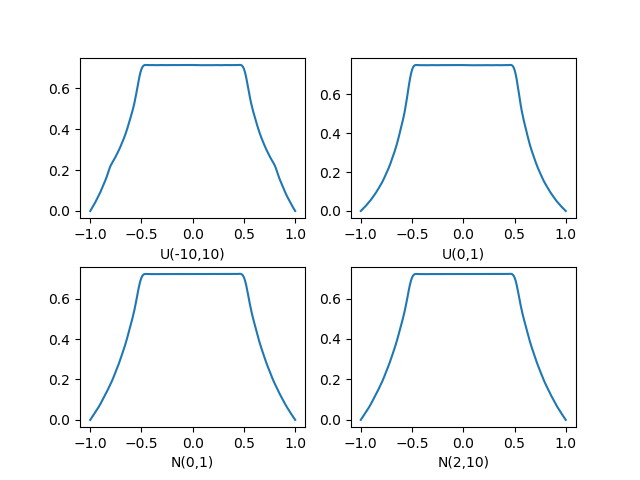
\includegraphics[scale=0.75]{Code/pics/several_examples}
\end{center}
\caption{Half-precision relative error distribution for four typical input distributions}
\label{fig:errdist}
\end{figure}

In fact, we will derive a \emph{single} density function which gives a good approximation of the error distribution \emph{for any sufficiently regular input distribution}. We will call this distribution the \emph{typical error distribution}.

We start by examining the quantity
\[
\one_{\fintvl[z]}\left(\frac{z}{1-tu}\right)
\]
which appears in \eqref{eq:pdf}. Given a $t\in\left[-1,1\right]$, we determine which floating point numbers $z\in\F\setminus\{-\infty,0,\infty\}$ make $\one_{\fintvl[z]}\left(\frac{z}{1-tu}\right)=1$. We will write floating point numbers $z\in\F$ in the form
\[
z=z(s,e,k):=(-1)^s ~ 2^e \left(1+\frac{k}{2^p}\right)
\]
where $s\in\{0,1\}$, $e$ ranges from $emin=1-n$ to $emax=n$ and $k$ ranges from 0 to $2^p-1$ (and represents the mantissa). We can explicitly compute $\floor{z}$ and $\ceil{z}$. When $s=0$ we have:
\begin{align}
\floor{z}=
\begin{cases}
2^{e-1} & \text{if }s=0, e=emin, k=0\\
2^{e-1}\left(1+\frac{2^{p+1}-1}{2^{p+1}}\right) & \text{if }s=0, e>emin, k=0\\
2^e\left(1+\frac{2k-1}{2^{p+1}}\right) & \text{else}
\end{cases}
\end{align}
and
\begin{align}
\ceil{z}=\begin{cases}
z&\text{if }s=0, e=n, k=2^p-1\\
2^e\left(1+\frac{2k+1}{2^{p+1}}\right) & \text{else}
\end{cases}
\end{align}
For $s=1$ note simply that
\begin{align}
\floor{-z}=-\ceil{z}\qquad\text{and}\qquad\ceil{-z}=-\floor{z}\label{eq:minz}
\end{align}
Since $u=2^{-(p+1)}$, when $s=0$ the condition $\floor{z}\leq \frac{z}{1-tu}\leq \ceil{z}$ becomes:
\begin{enumerate}
\item If $e=emin, k=0$:
\begin{align*}
2^{e-1}\left(1-\frac{t}{2^{p+1}}\right)\leq 2^e\leq 2^e\left(1+\frac{1}{2^{p+1}}\right)\left(1-\frac{t}{2^{p+1}}\right)
\end{align*}
from which we get
\begin{align}
-1\leq t\leq\frac{2^{p+1}}{2^{p+1}+1}\label{eq:trange1}
\end{align}
\item If $e>emin, k=0$:
\[
2^e\left(1-\frac{1}{2^{p+2}}\right)\left(1-\frac{t}{2^{p+1}}\right)\leq 2^e\leq 2^e\left(1+\frac{1}{2^{p+1}}\right)\left(1-\frac{t}{2^{p+1}}\right)
\]
from which we get:
\begin{align}
-\frac{2^{p+1}}{2^{p+2}-1}\leq t\leq \frac{2^{p+1}}{2^{p+1}+1}\label{eq:trange2}
\end{align}
\item If $e=n, k=2^p-1$:
\[
2^e\left(1+\frac{2(2^p-1)-1}{2^{p+1}}\right)\left(1-\frac{t}{2^{p+1}}\right)\leq 2^e\left(1+\frac{2^p-1}{2^p}\right) \leq 2^e\left(1+\frac{2^p-1}{2^p}\right)\left(1-\frac{t}{2^{p+1}}\right)
\]
from which we get
\begin{align}
-\frac{2^{p+1}}{2^{p+2}-3}\leq t\leq 0\label{eq:trange3}
\end{align}

\item Else: 
\begin{align*}
2^e\left(1+\frac{2k-1}{2^p}\right)\left(1-\frac{t}{2^p}\right)\leq 2^e\left(1+\frac{k}{2^p}\right)\leq 2^e\left(1+\frac{2k+1}{2^p}\right)\left(1-\frac{t}{2^p}\right)
\end{align*}
from which we get:
\begin{align}
-\frac{2^{p+1}}{2^{p+1}+2k-1}\leq t\leq \frac{2^{p+1}}{2^{p+1}+2k+1}\label{eq:trange4}
\end{align}
\end{enumerate}
The case for $s=1$ can then be derived from \eqref{eq:minz}:
\[
\floor{-z}\leq \frac{-z}{1-tu}\leq \floor{-z} \qquad\Leftrightarrow\qquad -\ceil{z}\leq \frac{-z}{1-tu}\leq -\floor{z} \qquad\Leftrightarrow\qquad \floor{z}\leq \frac{z}{1-tu}\leq \ceil{z}
\]
The bounds $t_{min}$ and $t_{max}$ of \eqref{eq:trange1}-\eqref{eq:trange4} are reached when the following relations are satisfied:
\begin{align*}
&\frac{1}{1-t_{max}u}=\frac{\ceil{z}}{z} & \frac{1}{1-t_{min}u}=\frac{\floor{z}}{z} & &\text{when } z\geq 0\\
&\frac{1}{1-t_{min}u}=\frac{\ceil{z}}{z} & \frac{1}{1-t_{max}u}=\frac{\floor{z}}{z} & &\text{when } z\leq 0
\end{align*}
It follows that 
\begin{align*}
\frac{\ceil{z}-\floor{z}}{\absv{z}}&=\left(\frac{1}{1-t_{max}u}-\frac{1}{1-t_{min}u}\right)=\frac{u(t_{max}-t_{min})}{(1-t_{max}u)(1-t_{min}u)}
\end{align*}
and thus
\begin{align}
\absv{z}u=\frac{(\ceil{z}-\floor{z})(t_{max}-t_{min})}{(1-t_{max}u)(1-t_{min}u)}\label{eq:absvzu}
\end{align}
where the coefficients $C(e,k):=\frac{(t_{max}-t_{min})}{(1-t_{max}u)(1-t_{min}u)}$ can be computed from Eqs. \eqref{eq:trange1}-\eqref{eq:trange4}.
\begin{enumerate}
\item  If $e=emin, k=0$:
\[
C(emin,0)=\frac{2^{p+1}+1}{2^p(2^{p+1}-1)}
\]
\item If $e>emin, k=0$:
\[
C(e,0)=\frac{2}{3}
\]
\item  If $e=n, k=2^p-1$:
\[
C(n,2^p-1)=\frac{3(2^{p+1}-1)}{2^{p+1}}
\]
\item Else:
\[
C(e,k)=\frac{2^p+k}{2^{p+1}}
\]
\end{enumerate}


We now use Eqs. \eqref{eq:trange1}-\eqref{eq:trange4} to express the possible values of $s,e,k$ for a given $t$. To check whether $k=0$ is possible one can simply use Eqs. \eqref{eq:trange1} and \eqref{eq:trange2} and to see if $e=n, k=2^p+1$ is possible one simply uses \eqref{eq:trange3}. For all other values of the exponent and the mantissa, \eqref{eq:trange4}, gives for $t\geq 0$:
\begin{align}
2^p\left(-\frac{1}{t}-1\right)+\frac{1}{2}\leq k\leq 2^p\left(\frac{1}{t}-1\right)-\frac{1}{2}\label{eq:kfromtpos}
\end{align}
and when $t\leq 0$:
\begin{align}
2^p\left(\frac{1}{t}-1\right)-\frac{1}{2}\leq k\leq 2^p\left(-\frac{1}{t}-1\right)+\frac{1}{2}\label{eq:kfromtneg}
\end{align}
Note that when $t\in\left[-\frac{1}{2},\frac{1}{2}\right]$, all combinations of $s,e,k$ are possible, and some mantissas will have to be excluded. For other values this will no longer be the case.
We have now enough details to describe the typical distribution. For $t\in\left[-\frac{1}{2},\frac{1}{2}\right]$, \eqref{eq:pdf} combined with \eqref{eq:absvzu} becomes 

\begin{align}
d(t)&=\sum_{z\in \F\setminus\{-\infty,0,\infty\}}f\left(\frac{z}{1-tu}\right) \frac{u\absv{z}}{(1-tu)^2}\nonumber
\\
=&\sum_{z\in \F\setminus\{-\infty,0,\infty\}}f\left(\frac{z}{1-tu}\right) \frac{1}{(1-tu)^2}\frac{(\ceil{z}-\floor{z})(t_{max}(z)-t_{min}(z))}{(1-t_{max}(z)u)(1-t_{min}(z)u)}&\nonumber
\\
=&\sum_{k=0}^{2^{p}-1}\left(\sum_{s=0}^1\sum_{e=emin}^{emax}f\left(\frac{z(e,s,k)}{1-tu}\right)\frac{C(e,k)(\ceil{z(e,s,k)}-\floor{z(e,s,k)})}{(1-tu)^2}\right)\nonumber 
\\
=&\sum_{k=0}^{2^p-1}\sum_{e=emin+1}^{emax-1}\sum_{s=0}^1 f\left(\frac{z(e,s,k)}{1-tu}\right)\frac{C(e,k)(\ceil{z(e,s,k)}-\floor{z(e,s,k)})}{(1-tu)^2}~+ \nonumber
\\
& \sum_{k=0}^{2^{p}-1}\sum_{s=0}^1 f\left(\frac{z(emin,s,k)}{1-tu}\right)\frac{C(emin,k)(\ceil{z(emin,s,k)}-\floor{z(emin,s,k)})}{(1-tu)^2}~+ \nonumber
\\
& \sum_{k=0}^{2^{p}-1}\sum_{s=0}^1 f\left(\frac{z(emax,s,k)}{1-tu}\right)\frac{C(emax,k)(\ceil{z(emax,s,k)}-\floor{z(emax,s,k)})}{(1-tu)^2}~+ \label{eq:pdf1/2}
\end{align}
Since $C(e,k)=\frac{2^p+k}{2^{p+1}}$ does not depend on $e$ when $emin<e<emax$ we can re-write the first term in the sum above as
\[
\sum_{k=0}^{2^p-1}\frac{C(e,k)}{(1-tu)^2}\sum_{e=emin+1}^{emax-1}\sum_{s=0}^1 f\left(\frac{z(e,s,k)}{1-tu}\right)(\ceil{z(e,s,k)}-\floor{z(e,s,k)})
\]
We now make three assumptions. Each assumption is formalized by exploiting the previous one(s).

\begin{enumerate}
\item \textbf{Assumption 1.} The probability density function is constant at the scale of the intervals between floating point numbers, i.e.
\[
\Pro{\Round(x)=z(e,s,k)}=\int_{\floor{z(e,s,k)}}^{\ceil{z(e,s,k)}} f(x)~dx \approx f\left(\frac{z(e,s,k)}{1-tu}\right)(\ceil{z(e,s,k)}-\floor{z(e,s,k)})
\]
for all values of $t$ such that $\one_{\fintvl[z]}\left(\frac{z}{1-tu}\right)=1$.
\item \textbf{Assumption 2.} The probability under $f$ of sampling a number whose rounding has exponent $emin$ or $emax$ is close to zero, i.e.
\[
 \sum_{k=0}^{2^{p}-1}\sum_{s=0}^1 f\left(\frac{z(emin,s,k)}{1-tu}\right)(\ceil{z(emin,s,k)}-\floor{z(emin,s,k)})\approx 0
\]
and
\[
 \sum_{k=0}^{2^{p}-1}\sum_{s=0}^1 f\left(\frac{z(emax,s,k)}{1-tu}\right)(\ceil{z(emax,s,k)}-\floor{z(emax,s,k)})\approx 0
\]
for all values of $t$ such that $\one_{\fintvl[z]}\left(\frac{z}{1-tu}\right)=1$
\item \textbf{Assumption 3.} When rounding a sample drawn from the distribution $f$, all mantissas are equally likely, i.e. for a given mantissa $k$
\[
\sum_{e=emin+1}^{emax-1}\sum_{s=0}^1 f\left(\frac{z(e,s,k)}{1-tu}\right)(\ceil{z(e,s,k)}-\floor{z(e,s,k)})\approx \frac{1}{2^p}
\]
for all values of $t$ such that $\one_{\fintvl[z]}\left(\frac{z}{1-tu}\right)=1$.
\end{enumerate}

Under these assumptions, \eqref{eq:pdf1/2} becomes
\begin{align}
d(t)&\approx\sum_{k=0}^{2^p-1}\frac{C(e,k)}{(1-tu)^2}\sum_{e=emin+1}^{emax-1}\sum_{s=0}^1 f\left(\frac{z(e,s,k)}{1-tu}\right)(\ceil{z(e,s,k)}-\floor{z(e,s,k)})\nonumber
\\
&\approx\frac{1}{2^p(1-tu)^2}\left(\frac{2}{3}+\sum_{k=1}^{2^p-1}\frac{2^p+k}{2^{p+1}}\right)\nonumber
\\
&=\frac{1}{2^p(1-tu)^2}\left(\frac{2}{3}+\frac{3(2^{p}-1)}{4}\right)\label{eq:pdf1/2ass}
\end{align}
If we assume further that $(1-tu)^2\approx 1$ we get that on $\left[-\frac{1}{2},\frac{1}{2}\right]$, $d(t)$ is equal to the constant $\frac{1}{2^p}\left(\frac{2}{3}+\frac{3(2^{p}-1)}{4}\right)$ which itself is approximated well by $\frac{3}{4}$ for sufficiently large precision levels $p$.

As shown by Eqs \eqref{eq:kfromtpos} \eqref{eq:kfromtneg}, when $\absv{t}>\frac{1}{2}$, not all mantissas in the sum \eqref{eq:pdf1/2} are possible, and for $t\geq 0$ \eqref{eq:pdf1/2ass} becomes 
\begin{align*}
d(t)&\approx\frac{1}{2^p(1-tu)^2}\left(\frac{2}{3}+\sum_{k=1}^{2^p(1/t-1)-1/2}\frac{2^p+k}{2^{p+1}}\right)
\\
&=\frac{1}{2^p(1-tu)^2}\left(\frac{2}{3}+\frac{1}{2}\floor{2^p(\frac{1}{t}-1)-\frac{1}{2}}+\frac{1}{2^{p+2}}(\floor{2^p(\frac{1}{t}-1)+\frac{1}{2}}\floor{2^p(\frac{1}{t}-1)-\frac{1}{2}})\right)
\end{align*}
where $\floor{2^p(\frac{1}{t}-1)-\frac{1}{2}}$ is the usual floor function applied to $2^p(\frac{1}{t}-1)-\frac{1}{2}$. Since we cannot give an analytic expression for this integer, it is useful to consider the limit behaviour for large precisions (\ie for $p\to\infty$) in which case the expression $\floor{2^p(1/t-1)-\frac{1}{2}}$ is very close to $2^p(\frac{1}{t}-1)-\frac{1}{2}$. The equation above then becomes
\[
d(t)\approx\frac{1}{(1-tu)^2}\left(\frac{1}{2}\left(\frac{1}{t}-1\right)+\frac{1}{4}\left(\frac{1}{t}-1\right)^2\right)
\]
in the limit where $p\to\infty$. The case where $t\leq -\frac{1}{2}$ is treated in the same way and yields the same asymptotic distribution. In the limit of large precisions and if we take $(1-tu)^2\approx 1$ we thus get the \emph{typical error distribution} with density function 
\begin{align}
d(t)=\begin{cases}
\frac{1}{(1-tu)^2}\left(\frac{1}{2}\left(\frac{1}{t}-1\right)+\frac{1}{4}\left(\frac{1}{t}-1\right)^2\right) & \text{if }t< \frac{-1}{2} \text{ or }t>\frac{1}{2}\\
\frac{3}{4}&\text{if }t\in\left[-\frac{1}{2} ,\frac{1}{2}\right]
\end{cases}\label{eq:typicalpdf}
\end{align}
We plot this density function $d(t)$ in Fig. \ref{fig:typical}. Note how close this approximate distribution is to the exact distributions plotted in Fig. \ref{fig:errdist}, even at half-precision level ($p=10$).



\begin{figure}[h!]
\begin{center}
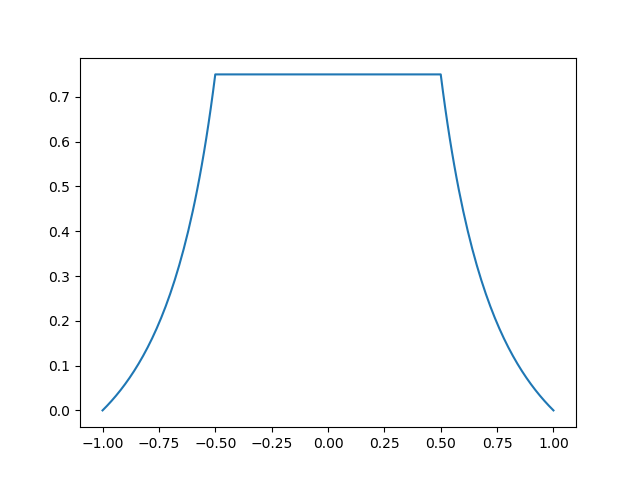
\includegraphics[scale=0.75]{Code/pics/typical_dist}
\end{center}
\caption{Typical distribution in the limit of large precision}
\label{fig:typical}
\end{figure}


\subsection{Characterising `sufficiently regular input distributions'}


%First we partition $\eR$ as the disjoint union
%\[
%\eR=\bigcup_{n\in \F}\Round\inv(n).
%\]
%On each element $x\in\Round\inv(n)$ of the partition we can compute the c.d.f. of the rounding error 
%\begin{align*}
%\mu\left(\left\{x\mid  x\in\Round\inv(n), \frac{\absv{x-\hat{x}}}{x}\leq t\right\}\right).
%\end{align*}
%where $t$ is of course bounded by $0\leq t\leq \uro$.
%Supposing first that $\hat{x}\geq 0$ and distinguishing the cases where $x<\hat{x}$ and $\hat{x}\leq x$ we get
%\begin{align*}
%&\mu\left(\left\{x\mid  x\in\Round\inv(n), \frac{\absv{x-\hat{x}}}{x}\leq t\right\}\right)\\
%=&\mu\left(\left\{x\mid x\in\Round\inv(n), x<\hat{x}, \frac{\hat{x}-x}{x}\leq t\right\}\right)+\mu\left(\left\{x\mid x\in\Round\inv(n), \hat{x}<x, \frac{x-\hat{x}}{x}\leq t\right\}\right)\\
%=&\mu\left(\left\{x\mid x\in\Round\inv(n), x<\hat{x}, \frac{\hat{x}}{x}-1\leq t\right\}\right)+\mu\left(\left\{x\mid x\in\Round\inv(n), \hat{x}<x, 1-\frac{\hat{x}}{x}\leq t\right\}\right)\\
%=&\mu\left(\left\{x\mid x\in\Round\inv(n), x<\hat{x}, \frac{\hat{x}}{1+t}\leq x\right\}\right)+\mu\left(\left\{x\mid x\in\Round\inv(n), \hat{x}<x, \frac{\hat{x}}{1-t}\geq x\right\}\right)\\
%=&\int_{\frac{\hat{x}}{1+t}}^{\hat{x}} f(u)~du+\int_{\hat{x}}^{\frac{\hat{x}}{1-t}}f(u)~du\qquad\qquad\text{where }\hat{x}=\Rep(n)\\
%=&\int_{\frac{\hat{x}}{1+t}}^{\frac{\hat{x}}{1-t}}f(u)~du
%\end{align*}
%Similarly, we get if $\hat{x}<0$ that
%\[
%\mu\left(\left\{x\mid x\in\Round\inv(n), \frac{\absv{x-\hat{x}}}{x}\leq t\right\}\right)=\int^{\frac{\hat{x}}{1+t}}_{\frac{\hat{x}}{1-t}}f(u)~du\qquad\qquad\text{where }\hat{x}=\Rep(n)\\
%\]
%We can now add up the contributions on each element of the partition to get
%\begin{align*}
%\mu\left(\left\{x\mid  \frac{\absv{x-\hat{x}}}{x}\leq t\right\}\right)=\sum_{n\in\F, \Rep(n)<0} \int^{\frac{\Rep(n)}{1+t}}_{\frac{\Rep(n)}{1-t}}f(u)~du +\sum_{n\in\F, \Rep(n)> 0} \int^{\frac{\Rep(n)}{1-t}}_{\frac{\Rep(n)}{1+t}}f(u)~du 
%\end{align*}


%Provided that $f$ is well-behaved (in a way which we shall make precise in an instant), we can provide a good approximation of each summand. For this we use the \emph{midpoint rule}:
%\begin{theorem}[Midpoint rule]
%Let $f\in C^2\left[a,b\right]$, then
%\begin{equation}
%\int_a^b f(u)~du =(b-a)f((a+b)/2)+ \varepsilon(a,b,f)\qquad\text{ where }\qquad \varepsilon(a,b,f)\leq\frac{\absv{b-a}^3}{24}\norm{f''}_{\infty} 
%\end{equation}
%\end{theorem}
%Assuming that terms of order $\uro^2$ (and thus $t^2\leq \uro^2)$ can be ignored we get from the midpoint rule that
%\begin{align*}
%\mu\left(\left\{x\mid  \frac{\absv{x-\hat{x}}}{x}\leq t\right\}\right)&=\sum_{n\in \F} \frac{2\Rep(n) t}{1+t^2}f\left(\frac{\Rep(n)}{1+t^2}\right)+\varepsilon\left(\frac{\Rep(n)}{1+t},\frac{\Rep(n)}{1-t},f\right)\\
%&\approx \sum_{n\in \F} 2\Rep(n) tf\left(\Rep(n)\right)+\varepsilon\left(\frac{\Rep(n)}{1+t},\frac{\Rep(n)}{1-t},f\right)\\
%&= \sum_{n\in \F}2\Rep(n) \uro f(\Rep(n)) \frac{t}{\uro}+\varepsilon\left(\frac{\Rep(n)}{1+t},\frac{\Rep(n)}{1-t},f\right)\\
%&\approx \sum_{n\in \F} \frac{2\Rep(n) \uro}{1+u^2}f\left(\frac{\Rep(n)}{1+u^2}\right)\frac{t}{\uro}+\varepsilon\left(\frac{\Rep(n)}{1+t},\frac{\Rep(n)}{1-t},f\right)\\
%&=\frac{t}{\uro}\left(\int_{-\infty}^{\infty} f(u)~du -\sum_{\in\F}\varepsilon\left(\frac{\Rep(n)}{1+u},\frac{\Rep(n)}{1-u},f\right)\right)+\sum_{\in\F}\varepsilon\left(\frac{\Rep(n)}{1+t},\frac{\Rep(n)}{1-t},f\right)\\
%&=\frac{t}{\uro}\left(1-\sum_{\in\F}\varepsilon\left(\frac{\Rep(n)}{1+u},\frac{\Rep(n)}{1-u},f\right)\right)+\sum_{\in\F}\varepsilon\left(\frac{\Rep(n)}{1+t},\frac{\Rep(n)}{1-t},f\right)\\
%&=\frac{t}{\uro}+\frac{t}{\uro}\sum_{\in\F}\frac{\Rep(n)^3(u^3-t^3)}{3(1+t^2)^3(1+u^2)^3}\norm{f''}_{\infty,n}
%\end{align*}
%For the second term in the last line to be small it is necessary that $\norm{f''}_\infty$ decays fast enough. If we want this term to be smaller that $\uro^2$ we need $\norm{f''}_{\infty,n}<\frac{3}{\Rep(n)^3\uro}$. 
%
%Conclusion: if $f''(x)$ can be bounded from above by something of the order of $\frac{3}{x^3\uro}$, then 
%\[
%\mu\left(\left\{x\mid  \frac{\absv{x-\hat{x}}}{x}\leq t\right\}\right)\approx \frac{t}{\uro}
%\]
%in other words the distribution of relative errors is, to a very good approximation, uniform on the interval $\left[0,\uro\right]$. If we can to include the sign of the error we would get an approximately uniform distribution on the interval $\left[-\uro,\uro\right]$ (maybe this is a slightly neater calculation). Since $f$ must be a density, it must decay very rapidly, and if the data is centred then it must decay very rapidly from 0, thus assuming $f''(x)<\frac{3}{x^3\uro}$ is not a very dramatic requirement.
%
%
%TODO: Deal with the interval $\fintvl[0]$, sort out notation for elements of $\F$ (cannot use $n$!).
\section{Modelling}



\subsection{Three models probabilistic models of floating-point arithmetic.}


\subsubsection{Model 1: correctly-rounded error model}
We introduce a first probabilistic model using the Markov chain $u$ on $\R$ defined as:
\[
u(x):=\begin{cases}
\Unif\left(\fintvl\right)& D\leq x\leq U\\
\delta_{-\infty}& x< D\\
\delta_{\infty} & x>U\end{cases}
\]
the uniform distribution on $\fintvl$ whose pdf is given by $f(t)=\frac{1}{(\ceil{x}-\floor{x})}\one_{\fintvl}(t)$. We now model floating-point arithmetic operations. Given $\diamond\in \{+,-,\times,/\}$ we define $\widehat{\diamond}:\F\times \F\to \F$ as the machine implementation of $\diamond$, and we also define $\diamond\fp$ as the Markov chain on $\R\times \R$ given by
\[
\diamond\fp:=u\circ\diamond.
\]
For example:
\[
x+\fp y:=\Unif\fintvl[x+y]
\]
It follows from the IEEE 754 standard (in particular the `correct rounding requirement') that the machine implementation $\hat{\diamond}$ and the probabilistic model $\diamond\fp$ must be related related via:
\[
(\Round)_\ast(x\diamond\fp y)=\delta_{\Round(x)~\widehat{\diamond}~\Round(y)}
\]
or, alternatively for $x,y\in\F$
\[
\Rep(x)\diamond\fp \Rep(y)=\Unif\left(\fintvl[\Rep(x~\hat{\diamond}~y)]\right)
\]

\begin{remark}
This model rounds correctly, but does not satisfy \eqref{eq:roundrelation}. Indeed, a number arbitrary close to $\ceil{x}$ can transition through $u$ to a number arbitrary close to $\floor{x}$, in which case the relative error is arbitrary close to $\frac{2u}{1-u}>2u>u$.
\end{remark}

\subsubsection{Model 2: uniform error model}

Any real number $x\in\R$ with $D< x< U$ satisfies (\cite[Th. 2.2]{higham2002accuracy}):
\begin{equation}\label{eq:roundrelation}
\Round(x)=x(1+\epsilon)\qquad\absv{\epsilon}\leq \uro
\end{equation}
where $\uro$ is the unit roundoff at precision $p$. We now introduce a model which consists in saying that $\epsilon$ is distributed uniformly on $\left[ -\uro,\uro\right]$, that it to say, each time a rounding operation occurs (explicitly or implicitly -- e.g. in a floating-point arithmetic operation), an error given by sampling uniformly from $\left[ -\uro,\uro\right]$ is added to the computation. More formally, we define the Markov chain on $\R$ given by
\[
v_{p}(x)=\begin{cases}
\Unif\left(\left[x(1-\uro),x(1+\uro)\right]\right) & D<x<U\\
\delta_{-\infty}& x< D\\
\delta_{\infty} & x>U
\end{cases}
\]
Note that the pdf of $\Unif\left(\left[x(1-\uro),x(1+\uro)\right]\right)$ is given by $f_v(t)=\frac{1}{2xu}\one_{\left[x(1-u),x(1+u)\right]}(t)$. 
Using this model we interpret the following program:
\begin{lstlisting}
/* Precondition: Inputs are distributed uniformly on [0,1] */

half x = ReadInput();
half y = ReadInput();
return (x+y) 
\end{lstlisting}
as the Markov kernel
\[
\xymatrix@C=10ex
{
\R^2 \ar[r]^{\langle v,v\rangle} & \R^2\ar[r]^{+} & \R\ar[r]^{v} & \R
}
\]
where we've denoted $v_{11}$ (for half-precision) as $v$ for notational clarity. To see why this is the case, note that $\mathtt{ReadInput()}$ preforms a rounding on each input, this explains the first kernel $\langle v,v\rangle$. The program then performs a floating-point addition, which by the IEEE 754 standard is equivalent to computing the addition in infinite precision (the deterministic kernel $+:\R^2\to\R$), follows by a rounding operation (the last $v:\R\to\R$).

\begin{remark}
This model does not round correctly in the sense that if $x$ is sufficiently close to $\ceil{x}$, then it is entirely possible for $v(x)$ to land in $\fintvl[y]$, where $y=\cceil{\ceil{x}}$ is the  first floating-point representable number following $\ceil{x}$ (which therefore does not round to the same number as $x$), and similarly if $x$ is sufficiently close to $\floor{x}$.
\end{remark}



\subsubsection{Model 3: machine-representable model}

Our third model is defined using the Markov chain defined by
\[
w(x)=\Unif\left(\ffintvl\right)
\]
This rounding-model is a probabilistic version of the interval-arithmetic model of rounding provided by the tool Daisy \cite{darulova2018daisy}. Note that Markov kernel $w$ is defined exclusively with uniform distributions on intervals whose bounds are machine-representable. Using this rounding model, the program 
\begin{lstlisting}
/* Precondition: Inputs are distributed uniformly on [0,1] */

half x = ReadInput();
half y = ReadInput();
return (x+y) 
\end{lstlisting}
is interpreted as the Markov kernel
\[
\xymatrix@C=10ex
{
\R^2 \ar[r]^{\langle w,w\rangle} & \R^2\ar[r]^{+} & \R\ar[r]^{w} & \R
}
\]

\begin{remark}
This model does not always round correctly or provide tight error bounds.
\end{remark}

\subsection{The suggested work-flow:}

\paragraph{Input Data:}
\begin{enumerate}
\item A joint input distribution $\mu$ on the program's $k$ real variables. For simplicity's sake we assume that the variables are independent, \ie $\mu=\mu_1\times\ldots\times \mu_k$ with $\mu_k\in\Giry\R$ 
\item A program using a sequential composition of arithmetic operations $\{+,-,\times,\div,\min,\max,\sqrt{}\}$ only. Specifically
\[
\tt{prog:=p_n\circ\ldots\circ p_1 (x_1,\ldots,x_k)}
\]
with each $\tt{p}_i$ binary or unary.
\end{enumerate} 

\paragraph{Output:} the rounding-error distribution of the output.

\paragraph{Work-flow:}

\begin{enumerate}
\item If $\tt{p}_1$ takes as inputs the variables $\tt{x_i,x_j}$, compute 
\begin{align}
p_1:=\sem{\tt{p}_1}_\ast(\mu_i \times \mu_j)\label{eq:step1}
\end{align}
\item Compute the error distribution 
\begin{align}
e_1=E(p_1)\label{eq:step2}
\end{align}
\item Push $p_1$ through the kernel 
\begin{align}
q_1:=(k_1)_\ast(p_1)\qquad\text{ where }\qquad k_1: \R\to\R, \qquad x\mapsto x\ast(1+e_1)\label{eq:step3}
\end{align}
\end{enumerate}

Note that \eqref{eq:step3} is an arithmetic operation on two random variables/probability measures: $x\sim p_1$ and $e_1$. 


\subsection{Probabilistic floating-point arithmetic on probabilistic inputs.}


\subsubsection{Model 1}


Given two probability measure $\mu,\nu$ on the inputs of an arithmetic operation (i.e.\@ on $\R$), we can compute the probability of the output as the probability measure given by
\[
(\diamond\fp)_\ast(\mu\times\nu)=u_\ast\circ \diamond_\ast (\mu\times \nu)
\]
which assigns to an interval $\intvl{a,b}$ the probability
\begin{equation}\label{eq:noisyoperation}
\int_{-\infty}^{\infty} u(x)\left(\intvl{a,b}\right) ~d\diamond_\ast(\mu\times \nu)
\end{equation}
If we assume that $\mu,\nu$ are absolutely continuous w.r.t. the Lebesgue measure $\lambda$ we can find two density functions $\nicefrac{d\mu}{d\lambda}:=f_\mu,\nicefrac{d\nu}{d\lambda}:=f_\nu$ such that
\[
\mu(A)=\int_A f_\mu(x)~dx\qquad\text{and}\qquad\nu(A)=\int_A f_\nu(x)~dx
\]
The probability measure $\diamond_\ast(\mu\times \nu)$ is then absolutely continuous with respect to the Lebesgue measure and we can then compute its density (see \cite{springer1979algebra}) as:

\begin{align}
\frac{d(+)_\ast(\mu\times\nu)}{d\lambda}(t)&=\int_{-\infty}^{\infty} f_\mu(x)f_\nu(t-x)~dx\label{eq:pdfplus}\\
\frac{d(-)_\ast(\mu\times\nu)}{d\lambda}(t)&=\int_{-\infty}^{\infty} f_\mu(x)f_\nu(x-t)~dx\label{eq:pdfminus}\\
\frac{d(\times)_\ast(\mu\times\nu)}{d\lambda}(t)&=\int_{-\infty}^{\infty} \frac{1}{\absv{x}}f_\mu(x)f_\nu\left(\frac{t}{x}\right)dx\label{eq:pdftimes}\\
\frac{d(/)_\ast(\mu\times\nu)}{d\lambda}(t)&=\int_{-\infty}^{\infty} \absv{x}f_\mu(x)f_\nu(tx)dx\label{eq:pdfdiv}
\end{align}
From this we can compute \eqref{eq:noisyoperation}. Let $f$ be any of the densities above, \eqref{eq:noisyoperation} amounts to computing
\[
\int_a^b u(x)\left(\intvl{a,b}\right) f(x) ~dx
\]
Assume that $a,b$ are machine representable numbers and that $a\neq b$. Given $x\in \R$ there are four possibilities
\begin{enumerate}
\item $\fintvl \cap \intvl{a,b}=\emptyset$, i.e.\ $\ceil{x}<a$ or $b>\floor{x}$ in which case 
\[
u(x)\left(\intvl{a,b}\right)=0
\]
\item  $\floor{x}\leq a\leq \ceil{x}<b$ in which case
\[
u(x)\left(\intvl{a,b}\right)=\frac{\ceil{x}-a}{\ceil{x}-\floor{x}}
\]
\item $\fintvl \subseteq \intvl{a,b}$, i.e.\ $a<\floor{x}, \ceil{x}<b$ in which case
\[
u(x)\left(\intvl{a,b}\right)=1
\]
\item  $a< \floor{x}\leq b<\ceil{x}$ in which case
\[
u(x)\left(\intvl{a,b}\right)=\frac{b-\floor{x}}{\ceil{x}-\floor{x}}
\]
\end{enumerate}
Since we've assumed that $a<b$ are machine representable, as $x$ varies from $-\infty$ to $\infty$ each of the cases described above occur in the order 1.2.3.4.1. We can thus partition $\R$ into five intervals. 
\begin{enumerate}
\item On $\left(-\infty,\floor{a}\right)$ we have $\ceil{x}<a$ and thus
\[
\int_{-\infty}^{\floor{a}} u(x)\left(\intvl{a,b}\right) f(x) ~dx=0
\]
\item On $\fintvl[a]$ we have $\floor{x}=\floor{a}\leq a\leq \ceil{a}=\ceil{x}$ and thus
\[
\int_{\floor{a}}^{\ceil{a}} u(x)\left(\intvl{a,b}\right) f(x) ~dx=\frac{\ceil{a}-a}{\ceil{a}-\floor{a}}\int_{\floor{a}}^{\ceil{a}}  f(x) ~dx
\]
\item On $\left(\ceil{a},\floor{b}\right)$ we have  i.e.\ $a<\floor{x}, \ceil{x}<b$ and thus
\[
\int_{\ceil{a}}^{\floor{b}} u(x)\left(\intvl{a,b}\right) f(x) ~dx=\int_{\ceil{a}}^{\floor{b}} f(x)~dx
\]
(Note that if $b$ is the next machine representable number after $a$ we have $\left(\ceil{a},\floor{b}\right)=\emptyset$ and this case drops out.)
\item On $\fintvl[b]$ we have $\floor{x}=\floor{b}\leq b\leq \ceil{b}=\ceil{x}$ and thus
\[
\int_{\floor{b}}^{\ceil{b}} u(x)\left(\intvl{a,b}\right) f(x) ~dx=\frac{b-\floor{b}}{\ceil{b}-\floor{b}}\int_{\floor{b}}^{\ceil{b}}  f(x) ~dx
\]
\item Finally, on $\left(\ceil{b},\infty\right)$ we have
\[
\int_{\ceil{b}}^{\infty} u(x)\left(\intvl{a,b}\right) f(x) ~dx=0
\]
\end{enumerate}

\noindent It follows that when $a<b$ are machine representable we can write \eqref{eq:noisyoperation} as
\begin{align*}
\int_{-\infty}^{\infty} u(x)\left(\intvl{a,b}\right) ~d\diamond_\ast(\mu\times \nu)=\frac{\ceil{a}-a}{\ceil{a}-\floor{a}}\int_{\floor{a}}^{\ceil{a}}  f(x) ~dx + \int_{\ceil{a}}^{\floor{b}} f(x)~dx +
\frac{b-\floor{b}}{\ceil{b}-\floor{b}}\int_{\floor{b}}^{\ceil{b}}  f(x) ~dx
\end{align*}
We can also compute the pdf of the probability measure $(\diamond\fp)_\ast(\mu\times \nu)$ defined by \eqref{eq:noisyoperation}. We have
\begin{align*}
(\diamond\fp)_\ast(\mu\times \nu)((-\infty,t))&=\int_{-\infty}^\infty u(x)(-\infty,t))f(x) ~dx\\
&=\int_{-\infty}^\infty \int_{-\infty}^t \frac{1}{\ceil{x}-\floor{x}} \one_{\fintvl}(y) f(x) ~dy dx\\
&=\int_{-\infty}^t\int_{-\infty}^\infty\frac{1}{\ceil{x}-\floor{x}} \one_{\fintvl}(y) f(x) ~dx dy
\end{align*}
where the last step is imply an application of Fubini's theorem. It follows that
\begin{align*}
\frac{d}{dt}(\diamond\fp)_\ast(\mu\times \nu)((-\infty,t))&=\int_{-\infty}^\infty\frac{1}{\ceil{x}-\floor{x}} \one_{\fintvl}(t) f(x) ~dx\\
&=\int_{\floor{t}}^{\ceil{t}}\frac{f(x)}{\ceil{t}-\floor{t}} ~dx
\end{align*}
This holds for \emph{any} initial density, in other words if $\mu$ is a probability measure with Lebesgue density $\nicefrac{d\mu}{d\lambda}=f$, then $u_\ast(\mu)$ has density
\begin{equation}
\frac{du_\ast(\mu)}{d\lambda}(t)=\int_{\floor{t}}^{\ceil{t}}\frac{f(x)}{\ceil{t}-\floor{t}} ~dx \label{eq:updf}
\end{equation}

\subsubsection{Model 2}

\subsection{Quantization operators }



The Markov chain $u$ defines a linear operator acting on measures on $\R$ via 
\[
Q: \Mes(\R)\to\Mes(\R), \mu\mapsto u_\ast(\mu)
\]
If a measure $\mu$ on $\R$ is absolutely continuous w.r.t. to the Lebesgue measure $\lambda$, then the operator $Q$ transform its density according to \eqref{eq:updf}, i.e.
\[
\frac{dQ(\mu)}{d\lambda}(t)=\int_{\floor{t}}^{\ceil{t}} \frac{1}{\ceil{t}-\floor{t}} \frac{d\mu}{d\lambda}~d\lambda 
\] 
We note immediately that $\frac{dQ(\mu)}{d\lambda}$ is piecewise constant, in fact constant over each interval $\fintvl[\Rep(i)], i\in \F$, which is why we will call $Q$ the $\F$-quantization operator, or simply the quantization operator if there is no ambiguity about $n,p$.

\subsection{Arithmetic of quantized distributions}

We compute \eqref{eq:pdfplus}-\eqref{eq:pdfdiv} for pdfs. It is clear from \eqref{eq:updf} that these are piecewise constant, i.e. a quantized pdf can always be expressed as a weighted sum of indicator functions:
\[
\sum_{i=1}^N \alpha_i \one_{\left[a_i,b_i\right]}
\]
Let us therefore start by computing \eqref{eq:pdfplus}-\eqref{eq:pdfdiv} for (scaled) indicator functions.

\subsubsection{Sums}
We denote by $\oplus$ the convolution of \eqref{eq:pdfplus} and we first compute the convolution of two weighted indicators:
\begin{align*}
\alpha\one_{[a,b]}\oplus\beta\one_{[c,d]}(t)& =\int_{-\infty}^\infty\alpha\one_{[a,b]}(x)\beta\one_{[c,d]}(t-x)dx \\
&=\alpha\beta\int_a^b \one_{[c,d]}(t-x)~dx\\
&= \begin{cases}
\alpha\beta(b-a)&c+b\leq t\text{ and }t\leq d+a\\
\alpha\beta((d+b)-t) & c+b\leq t\text{ and } d+a\leq t \\
\alpha\beta(t-(a+c)) & t\leq c+b\text{ and }t\leq d+a\\
\alpha\beta(d-c) & t\leq c+b\text{ and } d+a\leq t\\
0 &\text{else}
\end{cases}
\end{align*}

Note that convolutions are commutative and it follows by linearity of integration that
\begin{align*}
\sum_{i=1}^N \alpha_i \one_{\left[a_i,b_i\right]} \oplus \sum_{i=1}^N \alpha_i \one_{\left[a_i,b_i\right]}(t)&=\sum_{i,j=1}^N \alpha_i\one_{[a_1,b_1]}\oplus\beta_j\one_{[c_j,d_j]}(t) \\
&= 2\sum_{i\leq j=1}^N \alpha_i\one_{[a_1,b_1]}\oplus\beta_j\one_{[c_j,d_j]}(t)
\end{align*}


\subsubsection{Differences}

In the same way as above we compute 
\begin{align*}
\alpha\one_{[a,b]}\ominus\beta\one_{[c,d]}(t)&=\int_{-\infty}^{\infty} \alpha\one_{[a,b]}(x)\beta\one_{[c,d]}(x-t)~dx\\
&=\alpha\beta\int_a^b \one_{[c,d]}(x-t)~dx\\
&=\begin{cases}
\alpha\beta(d-c)&\text{if }a-c\leq t\text{ and }t\leq b-d\\
\alpha\beta((b-c)-t) &\text{if }a-c\leq t\text{ and }b-d\leq t\\
\alpha\beta(t-(a-d)) & \text{if }t\leq a-c\text{ and }t\leq b-d\\
\alpha\beta(b-a) & \text{if } t\leq a-c\text{ and }b-d\leq t\\
0&\text{else}
\end{cases}
\end{align*}
Note that, just like substraction, $\ominus$ is not commutative.

\subsection{Multiplication}
For notational clarity we assume $\alpha=\beta=1$
\begin{align*}
\int_{-\infty}^\infty \frac{1}{\absv{x}}\one_{[a,b]}(x)\one_{[c,d]}\left(\frac{t}{x}\right)~dx = &\int_{a}^b \frac{1}{\absv{x}}\one_{[c,d]}\left(\frac{t}{x}\right)~dx\\
=& \int_{\min(a,0)}^{\min(b,0)}\frac{1}{\absv{x}}\one_{[c,d]}\left(\frac{t}{x}\right)~dx+\int_{\max(a,0)}^{\max(b,0)}\frac{1}{\absv{x}}\one_{[c,d]}\left(\frac{t}{x}\right)~dx\\
=& \int_{\min(a,0)}^{\min(b,0)}\frac{1}{\absv{x}}\one_{[\min(c,0),\min(d,0)]}\left(\frac{t}{x}\right)~dx+\int_{\min(a,0)}^{\min(b,0)}\frac{1}{\absv{x}}\one_{[\max(c,0),\max(d,0)]}\left(\frac{t}{x}\right)~dx \\
& +\int_{\max(a,0)}^{\max(b,0)}\frac{1}{\absv{x}}\one_{[\min(c,0),\min(d,0)]}\left(\frac{t}{x}\right)~dx+\int_{\max(a,0)}^{\max(b,0)}\frac{1}{\absv{x}}\one_{[\max(c,0),\max(d,0)]}\left(\frac{t}{x}\right)~dx\\
:= & A+B+C+D
\end{align*}

\paragraph{Term D:}
\begin{align*}
D& =\int_{\max(a,0)}^{\max(b,0)}\frac{1}{\absv{x}}\one_{[\max(c,0),\max(d,0)]}\left(\frac{t}{x}\right)~dx\\
&=\begin{cases}
\int_{\frac{t}{\max(d,0)}}^{\frac{t}{\max(c,d)}}\frac{1}{x}~dx=\log\max(d,0)-\log\max(c,0)&\text{if }\max(a,0)\leq \frac{t}{\max(d,0)}\leq \frac{t}{\max(c,0)}\leq \max(b,0)\\
0&\text{else}
\end{cases}
\end{align*}

\section{Computing instability probabilities}

We now show how to compute some simple instability probabilities.

\subsection{Programs with no operation}


\begin{lstlisting}
/* Precondition: Input is distributed uniformly on [0,1] */

half x = ReadInput();
if (x>0.25){
  return TRUE;}
else{
  return FALSE;} 
\end{lstlisting}

Let us call the program above $\tt Prog$ and assume that the input is a real number drawn randomly and uniformly from $\intvl{0,1}$. The function \texttt{ReadInput} rounds the input to a floating-point number in $\F$. The variable $\tt x$ is thus distributed according to
\[
(\Round)_\ast(\Unif(0,1))
\]
For $X\sim\Unif(0,1)$ we are interested in computing the probability of misclassification, i.e.\@
\[
\Pro{\mathtt{Prog}(X)=\mathtt{FALSE}\mid X> 0.25}
\]
This can be computed explicitly as
\begin{align*}
\Pro{\mathtt{Prog}(X)=\mathtt{FALSE}\mid X> 0.25}&=\frac{\Pro{\mathtt{Prog}(X)=\mathtt{FALSE} \wedge X> 0.25}}{\Pro{X> 0.25}}\\
&=\frac{\Pro{X\in \{x\mid\Round[5,10](x)\leq 0.25\wedge  x>0.25  \}}}{0.75}\\
&=\frac{\ceil{0.25}-0.25}{0.75}
\end{align*}

More generally if $X$ is distributed according to some density $f_X$ and $C$ is the machine-representable value of the threshold we have
\[
\Pro{\mathtt{Prog}(X)=\mathtt{FALSE}\mid X> C}=\frac{\int_C^{\ceil{C}} f_X(x)~dx}{\int_{x>C} f_X(x)~dx}
\]

%\[
%\xymatrix@C=12em
%{
%\R\ar[r]^{\Round[5,10]} & \F[5,10]\ar[r]^{->0.25} & \B
%}
%\]

\subsubsection*{b) Programs with one operation}

\newcommand{\rRound}{\mathrm{Round}}

\begin{lstlisting}
/* Precondition: Inputs are distributed uniformly on [0,1] */

half x = ReadInput();
half y = ReadInput();
if (x+y>0.25){
  return TRUE;}
else{
  return FALSE;} 
\end{lstlisting}

This time we want to compute:
\[
\Pro{\mathtt{Prog}(X,Y)=\mathtt{FALSE}\mid X+Y> C}.
\]
This is more complex because we model $\mathtt{Prog}(X,Y)$ by using $+\fp$. For notational clarity we define $\rRound:=\Rep\circ \Round$.
\begin{align*}
&\Pro{\mathtt{Prog}(X,Y)=\mathtt{FALSE}\mid X+Y> C}\\
:=&\Pro{(u\circ + \circ (\rRound\times \rRound))(X,Y)\in\{(-\infty,C]\}\mid X+Y>C}\\
=&\int_{C}^{\infty}\left( \int_{\R^2}(u\circ + \circ (\rRound\times \rRound))(x,y)(-\infty,C]
~\frac{\phi_\mu(x)\phi_\nu(y)}{\phi_\mu\ast\phi_\nu(z)}\delta(z-x-y) ~dx~dy\right)\phi_\mu\ast\phi_\nu(z)~dz\\
=&\int_{C}^{\infty} \int_{-\infty}^\infty (u\circ + \circ (\rRound\times \rRound))(x,z-x)(-\infty,C]~\phi_\mu(x)\phi_\nu(z-x)~dx~dz\\
=&\int_{C}^{\infty} \int_{-\infty}^\infty u(\rRound(x)+\rRound(z-x))(-\infty,C]\phi_\mu(x)\phi_\nu(z-x)~dx~dz 
\end{align*}
%Note that:
%\begin{itemize}
%\item $u(t)(-\infty,C]=0$ if $t>\ceil{C}$. Moreover, 
%\item $u(t)(-\infty,C]=\frac{C-\floor{C}}{\ceil{C}-\floor{C}}$ if $\floor{C}\leq t\leq \ceil{C}$
%\item $u(t)(-\infty,C]=1$ if $t<\floor{C}$
%\item $C\leq z$
%\end{itemize} 
%Note also that
%\begin{lemma}\label{lem:distrib}
%The following equivalences hold:
%\begin{enumerate}
%\item $\rRound(x)+\rRound(z-x)>\ceil{C}\Leftrightarrow z>\ceil{C}$
%\item $\rRound(x)+\rRound(z-x)<\floor{C}\Leftrightarrow z<\floor{C}$
%\end{enumerate}
%\end{lemma}
%\begin{proof}
%We have:
%\begin{align*}
%&\rRound(x)+\rRound(z-x)>\ceil{C}\\
%\Leftrightarrow & \floor{\rRound(x)+\rRound(z-x)}>\ceil{C}\\
%\Leftrightarrow &\floor{\rRound(\rRound(x)+\rRound(z-x))}>\ceil{C}\\
%\Leftrightarrow & (1-u)(\rRound(x)+\rRound(z-x))>\ceil{C}\\
%\Leftrightarrow & (1-u)\rRound(x)+(1-u)\rRound(z-x)>\ceil{C}\\
%\Leftrightarrow & \floor{\rRound(x)}+\floor{\rRound(z-x)}>\ceil{C}\\
%\Leftrightarrow & \floor{x}+\floor{z-x}>\ceil{C}\\
%\Leftrightarrow & (1-u)x+(1-u)(z-x)>\ceil{C}\\
%\Leftrightarrow &\floor{z}>\ceil{C}\\
%\Leftrightarrow & z>\ceil{C}
%\end{align*}
%and similarly for the second equivalence.
%\end{proof}
%
%From the first equivalence we get that $u(\rRound(x)+\rRound(z-x))(-\infty,C]=0$ when  $z>\ceil{C}$ and from the second equivalence we see that $u(\rRound(x)+\rRound(z-x))(-\infty,C]=1$ if $z<\floor{C}$, which contradicts $C\leq z$, i.e. this case does not present itself. Thus the only non-zero contribution is when 
%\[
%\floor{C}<\rRound(z)<\ceil{C}
%\]
%The integral above now become
%\begin{align*}
%\Pro{\mathtt{Prog}(X,Y)=\mathtt{FALSE}\mid X+Y> C}=&\int_C^{\ceil{C}}\int_{-\infty}^\infty \frac{C-\floor{C}}{\ceil{C}-\floor{C}}\phi_\mu(x)\phi_\nu(z-x)~dx~dz \\
%=&\int_C^{\ceil{C}}\frac{C-\floor{C}}{\ceil{C}-\floor{C}}~\phi_\mu\ast\phi_\nu(z)~dz
%\end{align*}
%
%\begin{remark}
%Lemma \ref{lem:distrib} does \textbf{not} hold for multiplication and division since it relies on the distributivity of $+$ over $\times$. It also does \textbf{not} hold for fixed point representation since it also relies on expressing $\floor{x}$ and $(1-u)x$. 
%\end{remark}
\subsection*{More than one operation}

Consider now a program of the shape
\begin{lstlisting}
/* Precondition: Inputs are distributed uniformly on [0,1] */

half x = ReadInput();
half y = ReadInput();
half z = ReadInput();
if (1+x+(y*z)/2>0.25){
  return TRUE;}
else{
  return FALSE;} 
\end{lstlisting}

The function $\mathtt{1+x+(y*z)/2}$ provides an over-approximation of the distribution of $\mathtt{1+x+(x*x)/2}$, a common approximation of $\mathtt{exp(x)}$. We can consider (1) the distribution of $\mathtt{1+x+(y*z)/2}$ and (2) the probability of misclassification.

Let's start with computing the distribution of $\mathtt{1+x+(y*z)/2}$. We define $\upsilon$ to be the uniform measure on $\intvl{0,1}$. The measure we're looking for is given by the pushforward of the measure $\upsilon\times\upsilon\times\upsilon$ through the sequence of (probabilistic) maps
\[
\xymatrix@C=12ex
{
\R^3\ar[r]^{\langle \id, \times\rangle} & \R^2\ar[r]^{\langle\id,\frac{-}{2}\rangle} & \R^2\ar[r]^{\langle\id,u\rangle} & \R^2 \ar[r]^{+} & \R\ar[r]^{-+1} &\R\ar[r]^{u}&\R
}
\]
Here we assume for simplicity's sake that we can do $(\cdot\times\cdot)/2$ and $1+\cdot+\cdot$ in one operation. We know that the pdf of $((\cdot \times \cdot)/2)_\ast(\upsilon\times\upsilon)$ is given via \eqref{eq:pdftimes} by
\begin{align*}
\phi(t)&=\frac{1}{2}\int_{-\infty}^\infty \frac{1}{\absv{x}} \one_{\intvl{0,1}}(x) \one_{\intvl{0,1}}\left(\frac{t}{x}\right)~dx\\
&=\frac{1}{2}\int_0^\infty \frac{1}{x}\one_{\intvl{0,1}}(x) \one_{\intvl{0,1}}\left(\frac{t}{x}\right)~dx+\int_{-\infty}^0 -\frac{1}{x}\one_{\intvl{0,1}}(x) \one_{\intvl{0,1}}\left(\frac{t}{x}\right)~dx\\
&=\frac{1}{2}\int_0^1 \frac{1}{x}\one_{\intvl{0,1}}\left(\frac{t}{x}\right)~dx\\
&=\frac{1}{2}\one_{\intvl{0,1}}(t)\int_t^1 \frac{1}{x}~dx \\
&=\frac{1}{2}\one_{\intvl{0,1}}(t) (-\log(t))
\end{align*}
And thus thus, the pdf of $(u\circ (\cdot \times \cdot)/2))_\ast(\upsilon\times\upsilon)$ is given via \eqref{eq:updf} by
\begin{align*}
\hat{\phi}(t)&=\sum_{i\in \Rep \left[\F\right]} \one_{\intvl{\floor{i},\ceil{i}}}(t) \int_{\floor{i}}^{\ceil{i}}\frac{\phi(x)}{\ceil{i}-\floor{i}} ~dx\\
&=\sum_{i\in \Rep \left[\F\right]\cap\intvl{0,1}}  \one_{\intvl{\floor{i},\ceil{i}}}(t) \frac{\ceil{i}(1-\log(\ceil{i})-\floor{i}(1-\log(\floor{i})}{\ceil{i}-\floor{i}}
\end{align*}
We can now compute the density of $(1+\cdot+\cdot)\ast$ applied to the product of $(u\circ (\cdot \times \cdot)/2))_\ast(\upsilon\times\upsilon)$  and $\upsilon$ via \eqref{eq:pdftimes}:
\begin{align*}
\psi(t)=\int_{-\infty}^\infty \hat{\phi}(x) \one_{\intvl{1,2}}(t-x)~dx
\end{align*}
\bibliographystyle{plain}
\bibliography{george} 
\end{document}